% Auto-generated: lecture page scans for unit 10
\section*{Lecture Pages (Unit 10)}
\addcontentsline{toc}{section}{Lecture Pages (Unit 10)}
\begin{figure}[p]
  \centering
  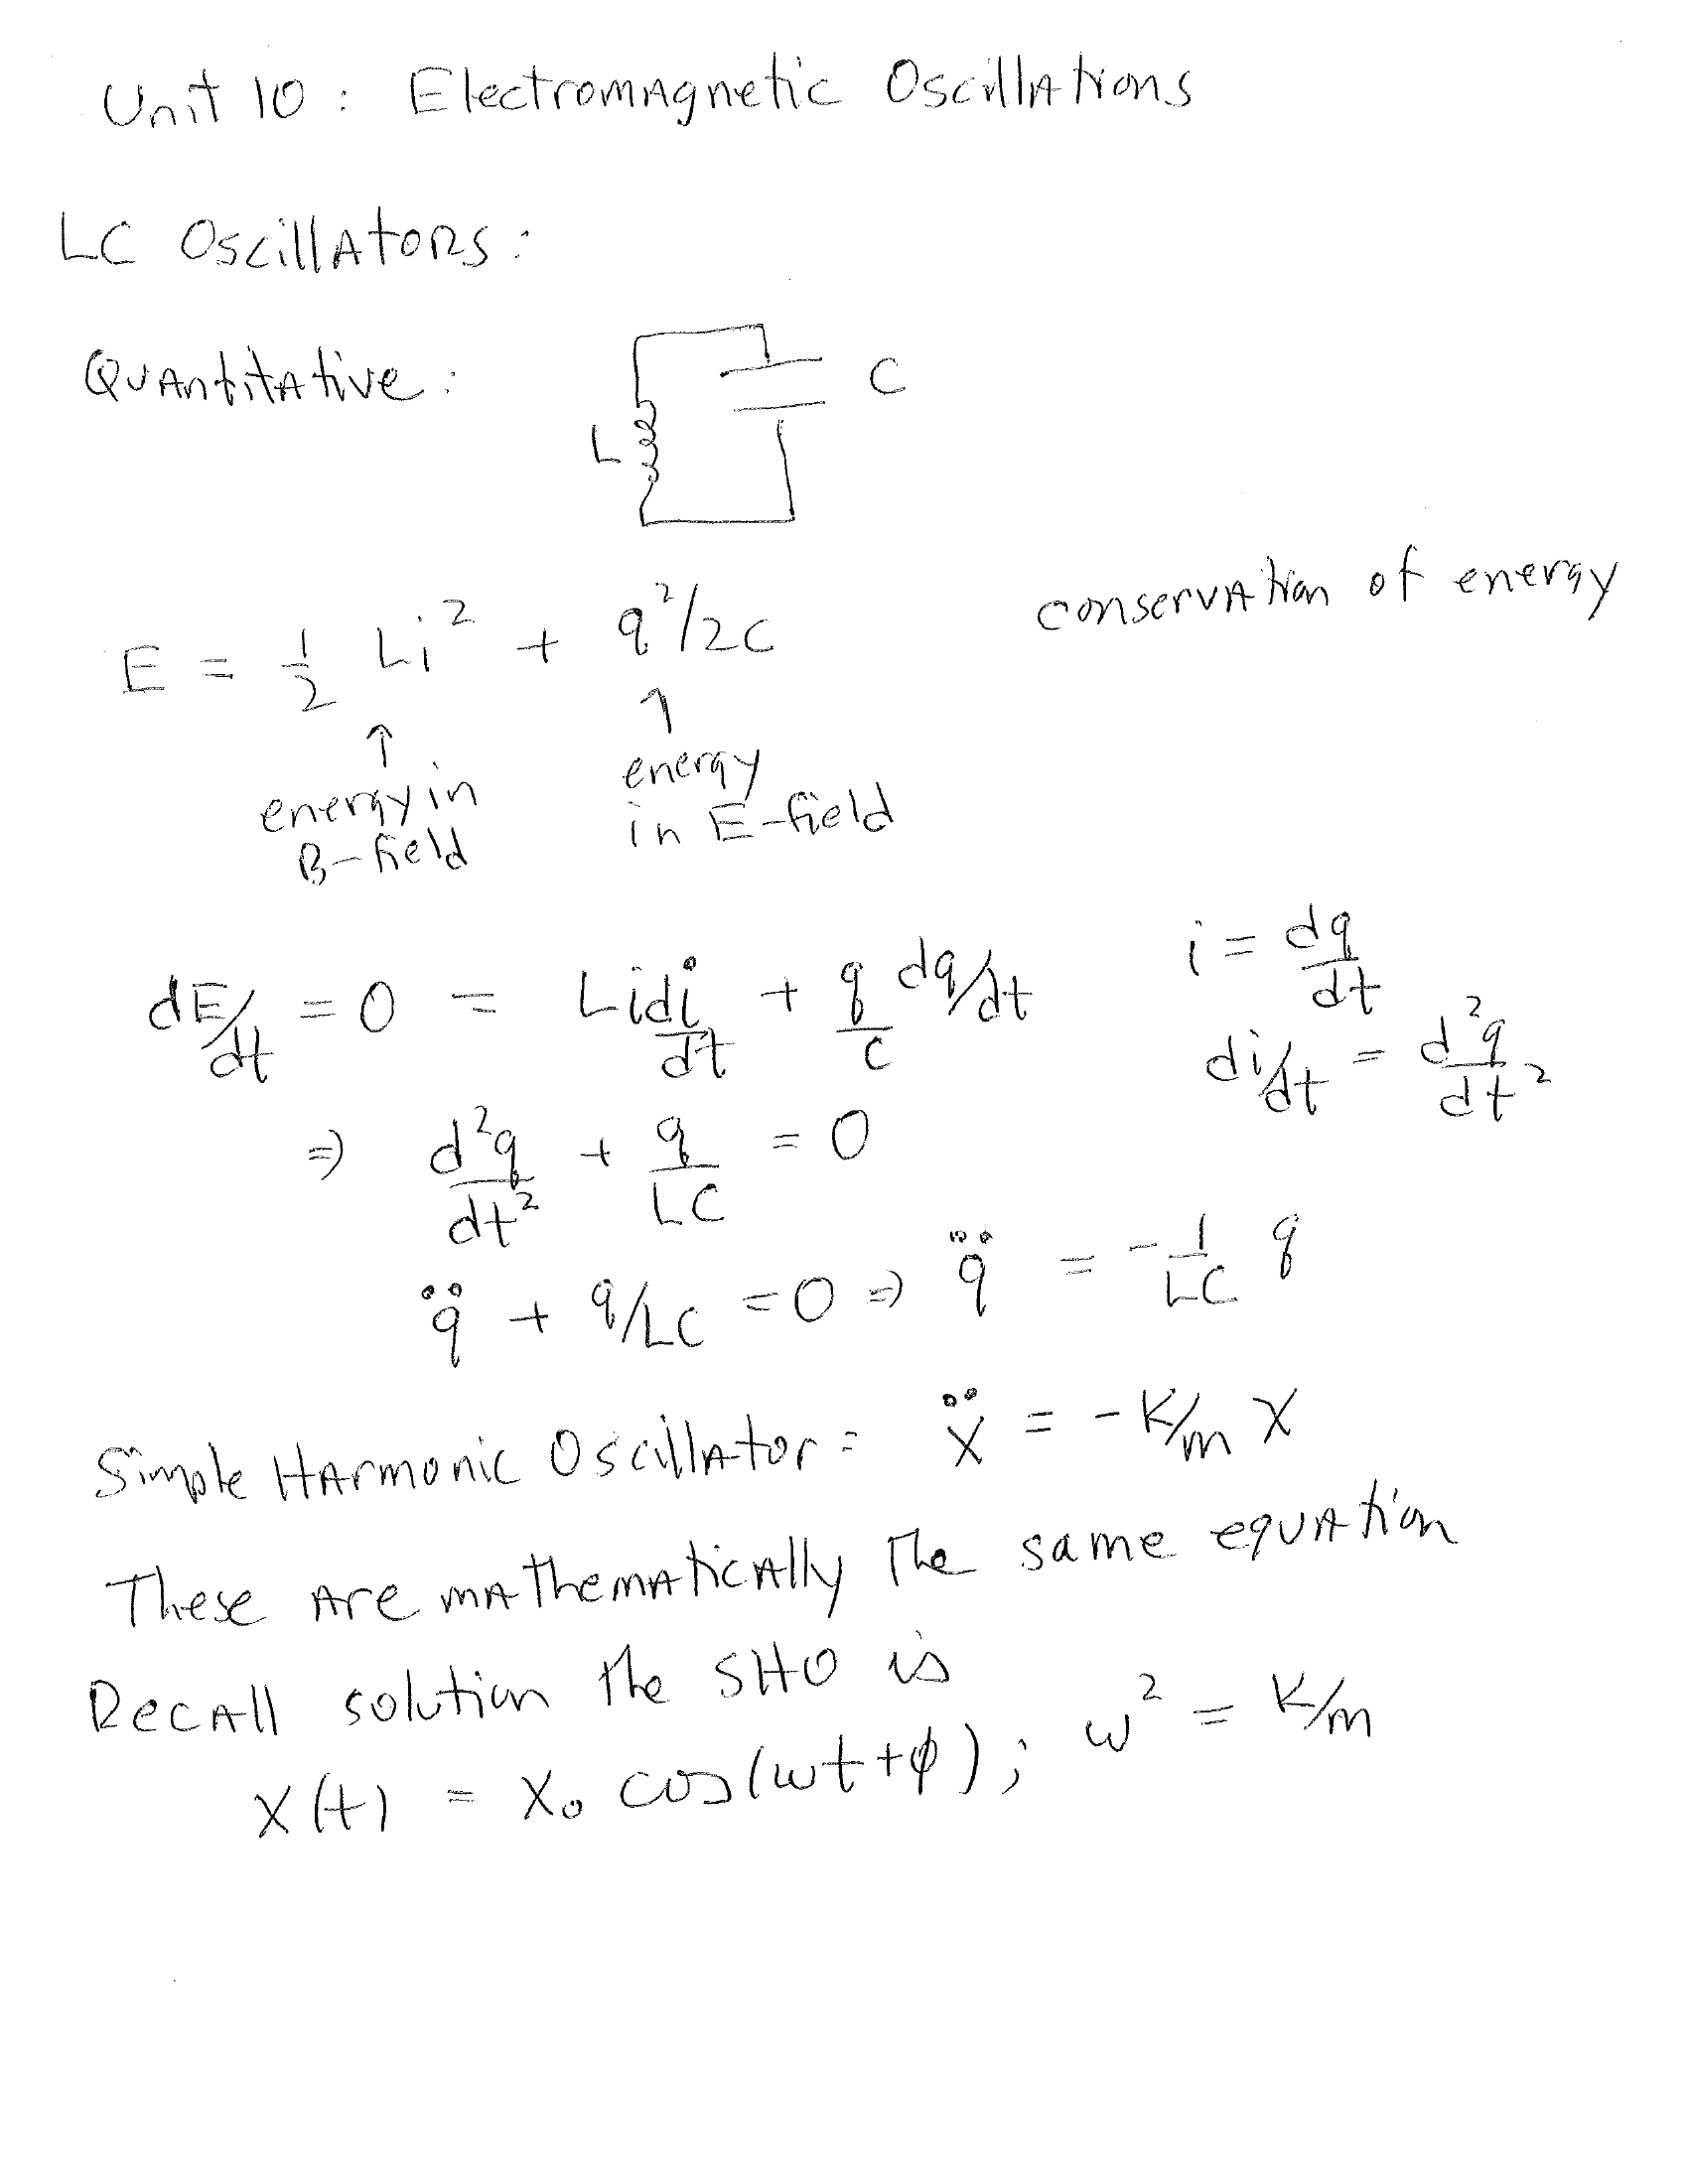
\includegraphics[width=0.9\textwidth,keepaspectratio]{figures/unit_10/page-1.png}
  \caption*{Unit 10, page 1}
\end{figure}
\clearpage
\begin{figure}[p]
  \centering
  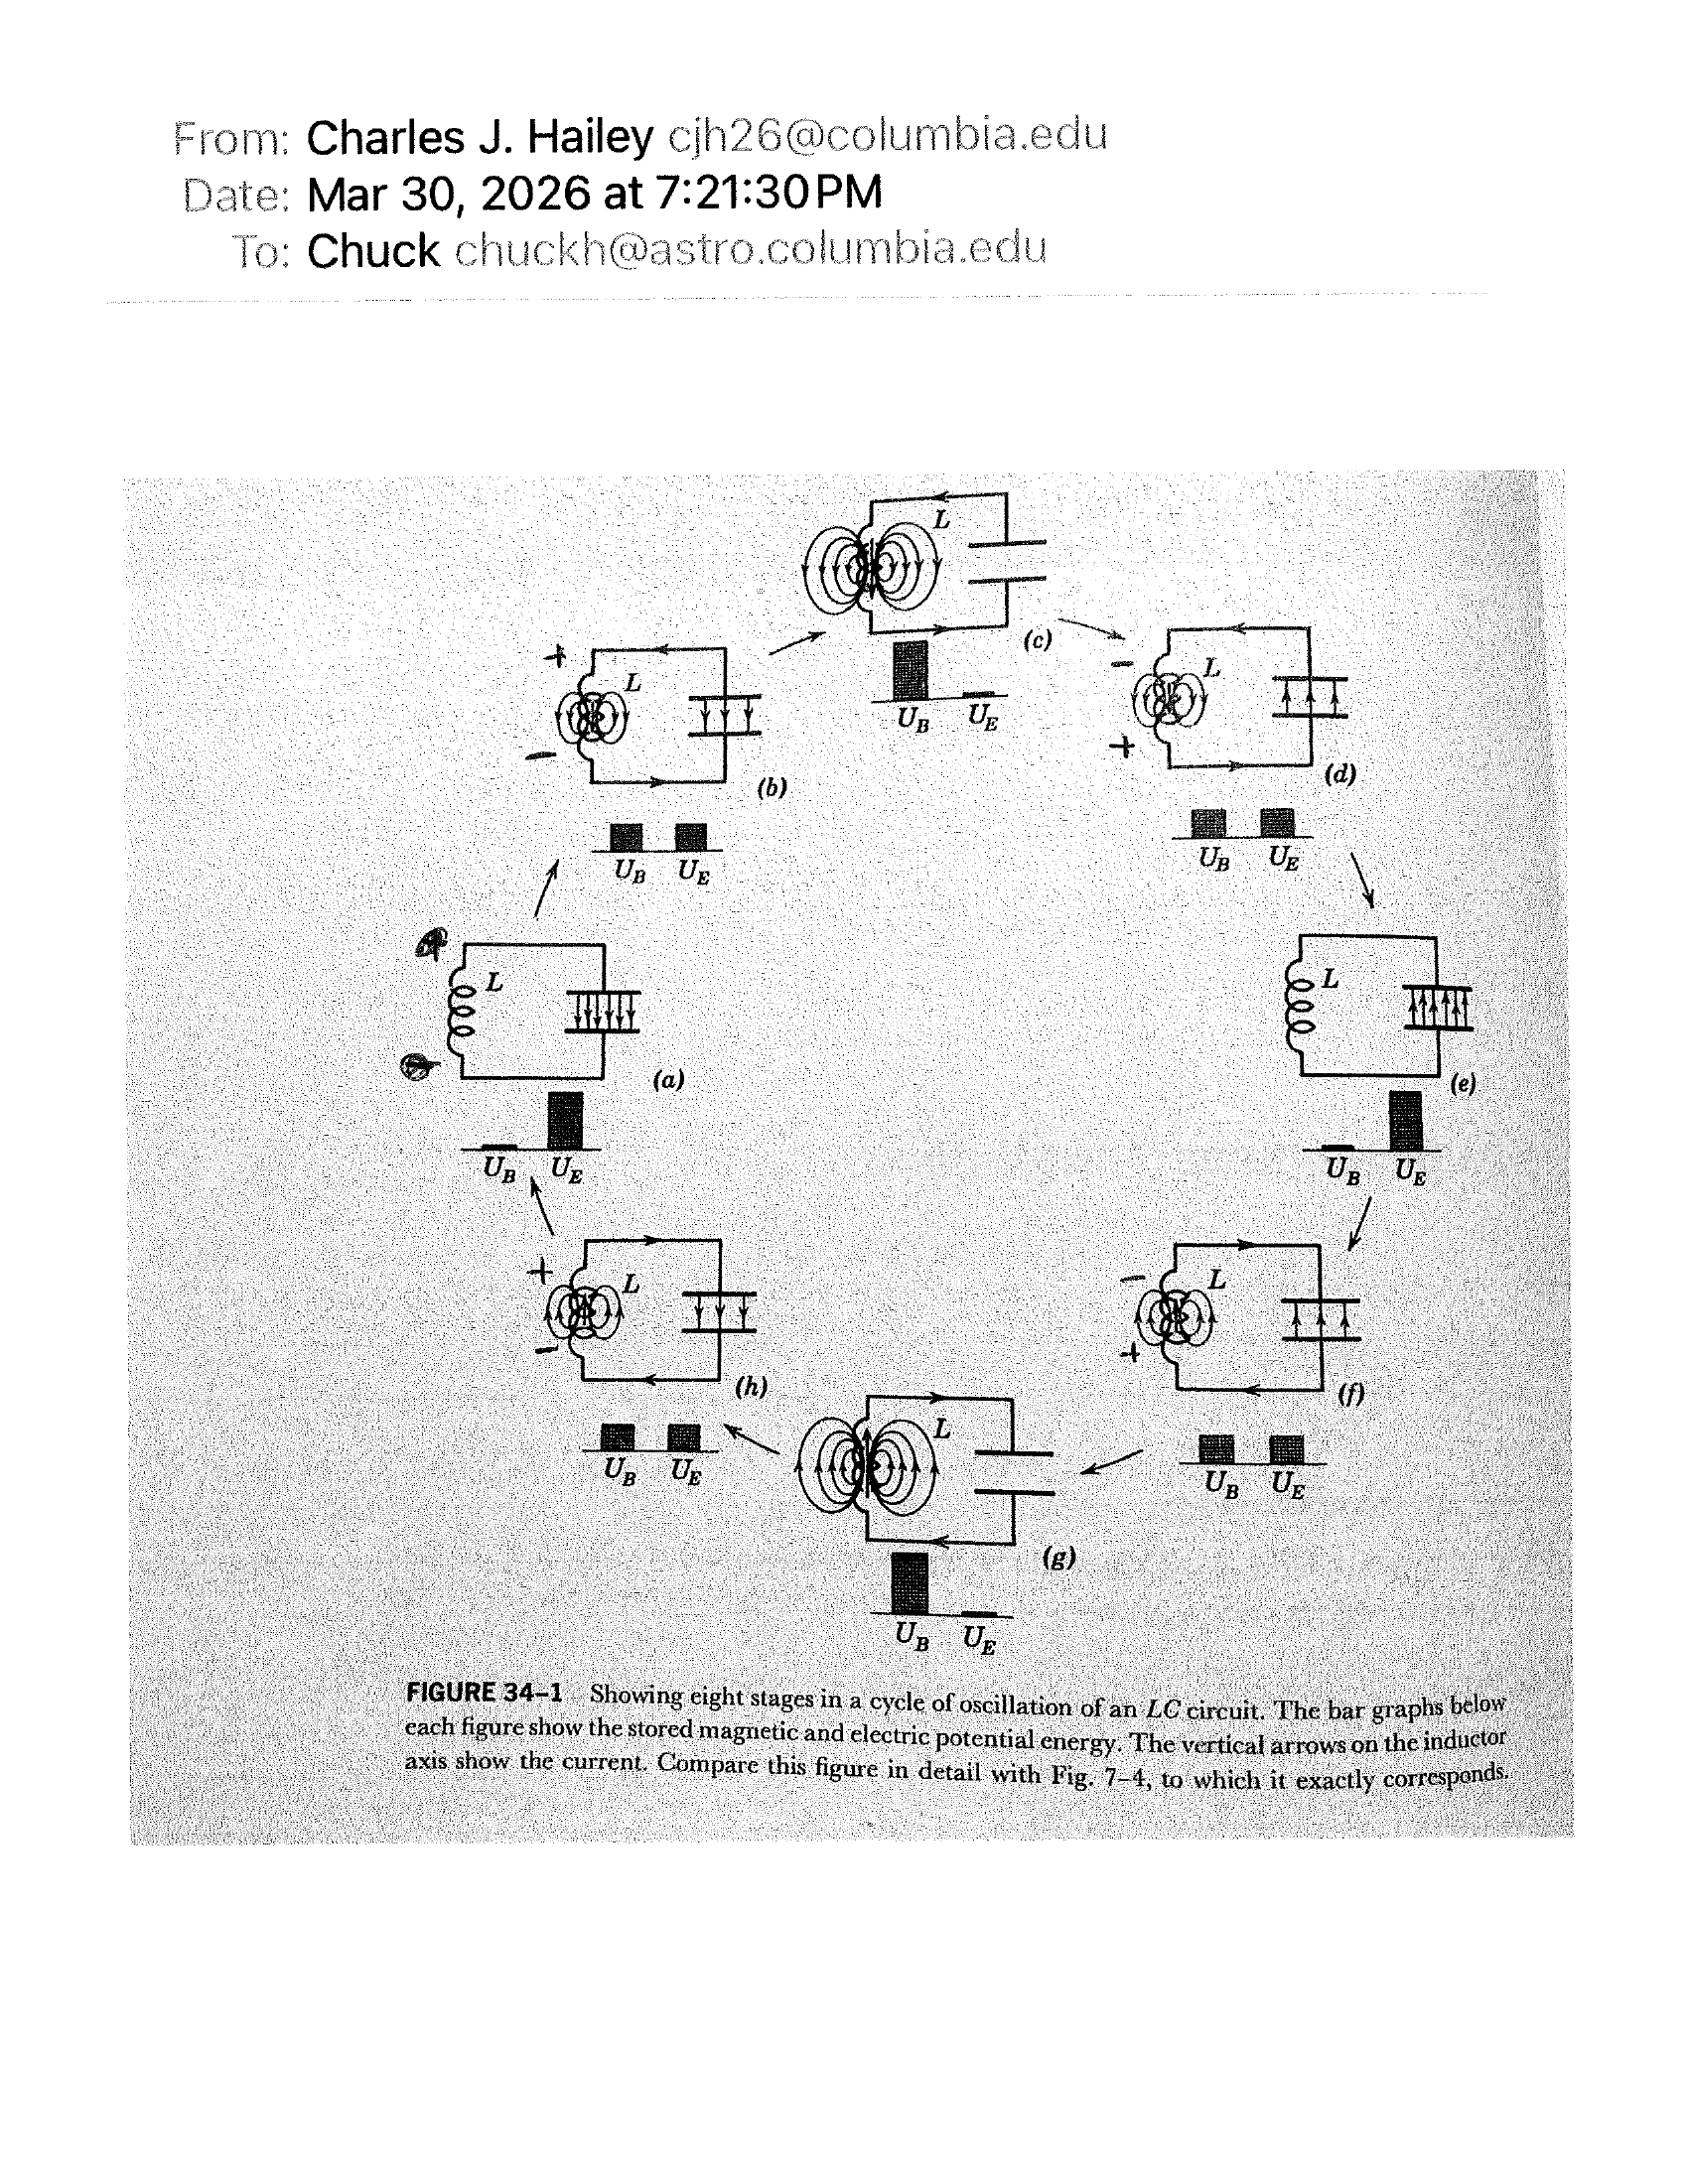
\includegraphics[width=0.9\textwidth,keepaspectratio]{figures/unit_10/page-2.png}
  \caption*{Unit 10, page 2}
\end{figure}
\clearpage
\begin{figure}[p]
  \centering
  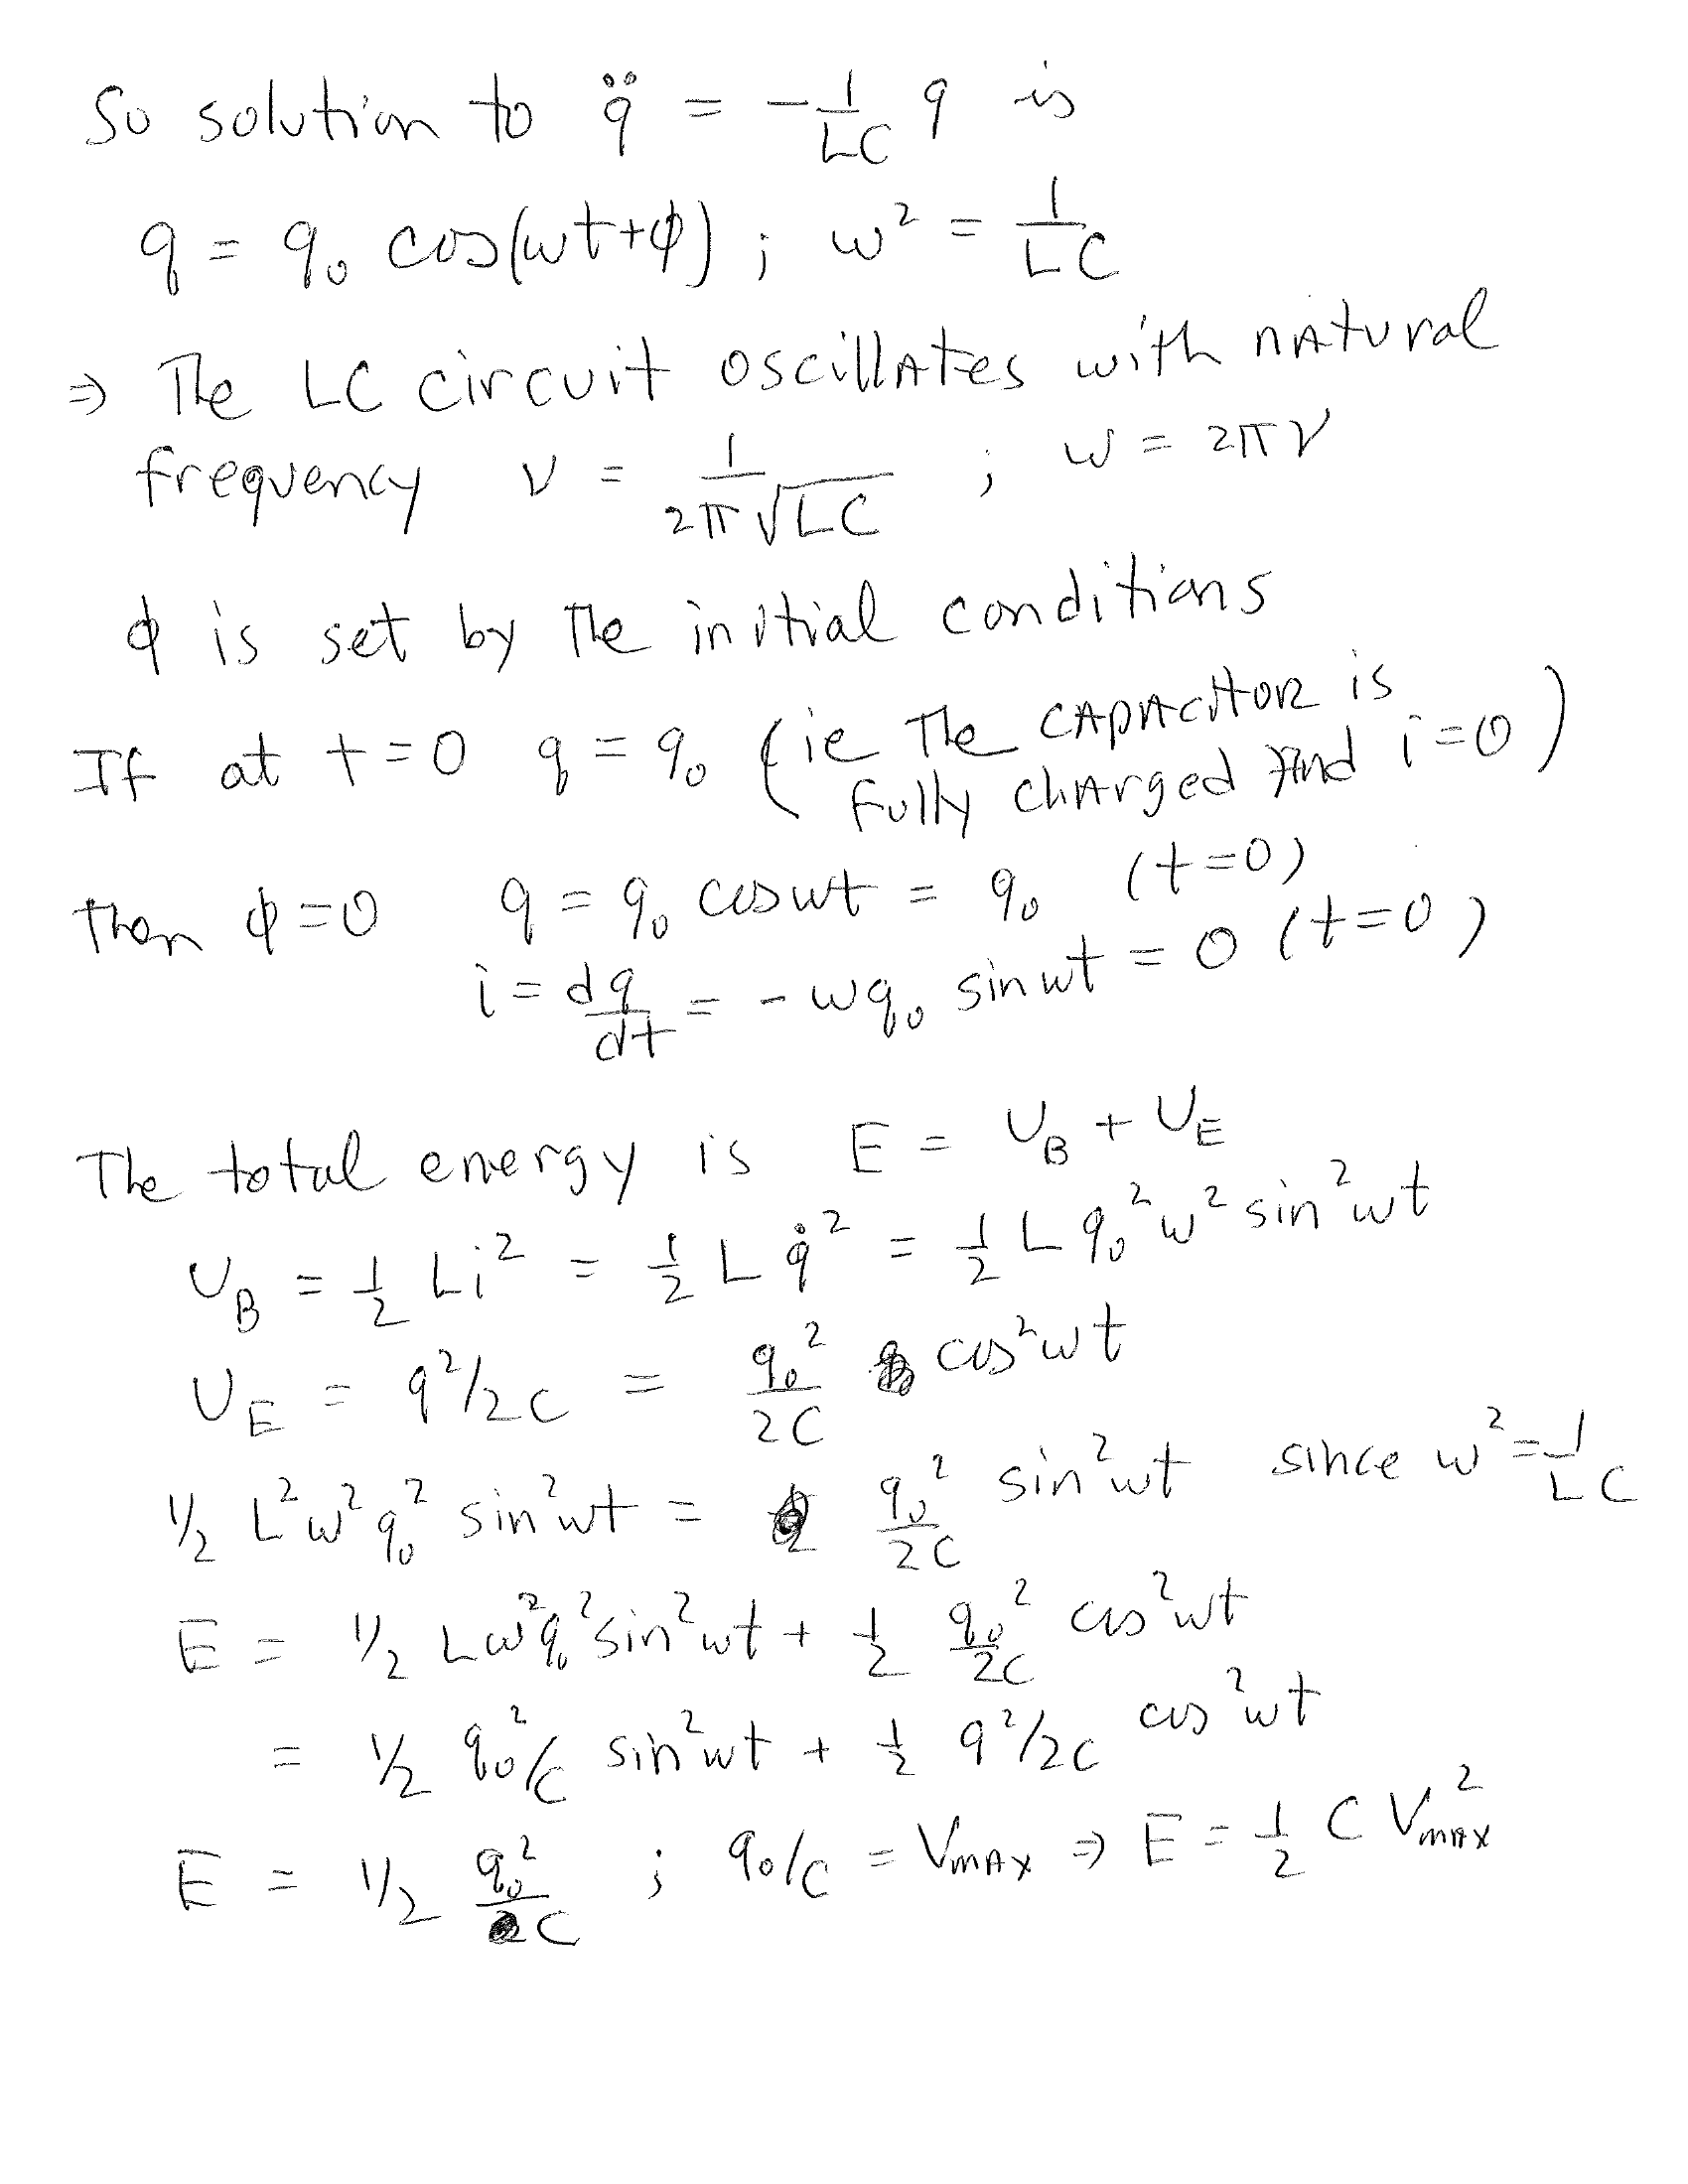
\includegraphics[width=0.9\textwidth,keepaspectratio]{figures/unit_10/page-3.png}
  \caption*{Unit 10, page 3}
\end{figure}
\clearpage
\begin{figure}[p]
  \centering
  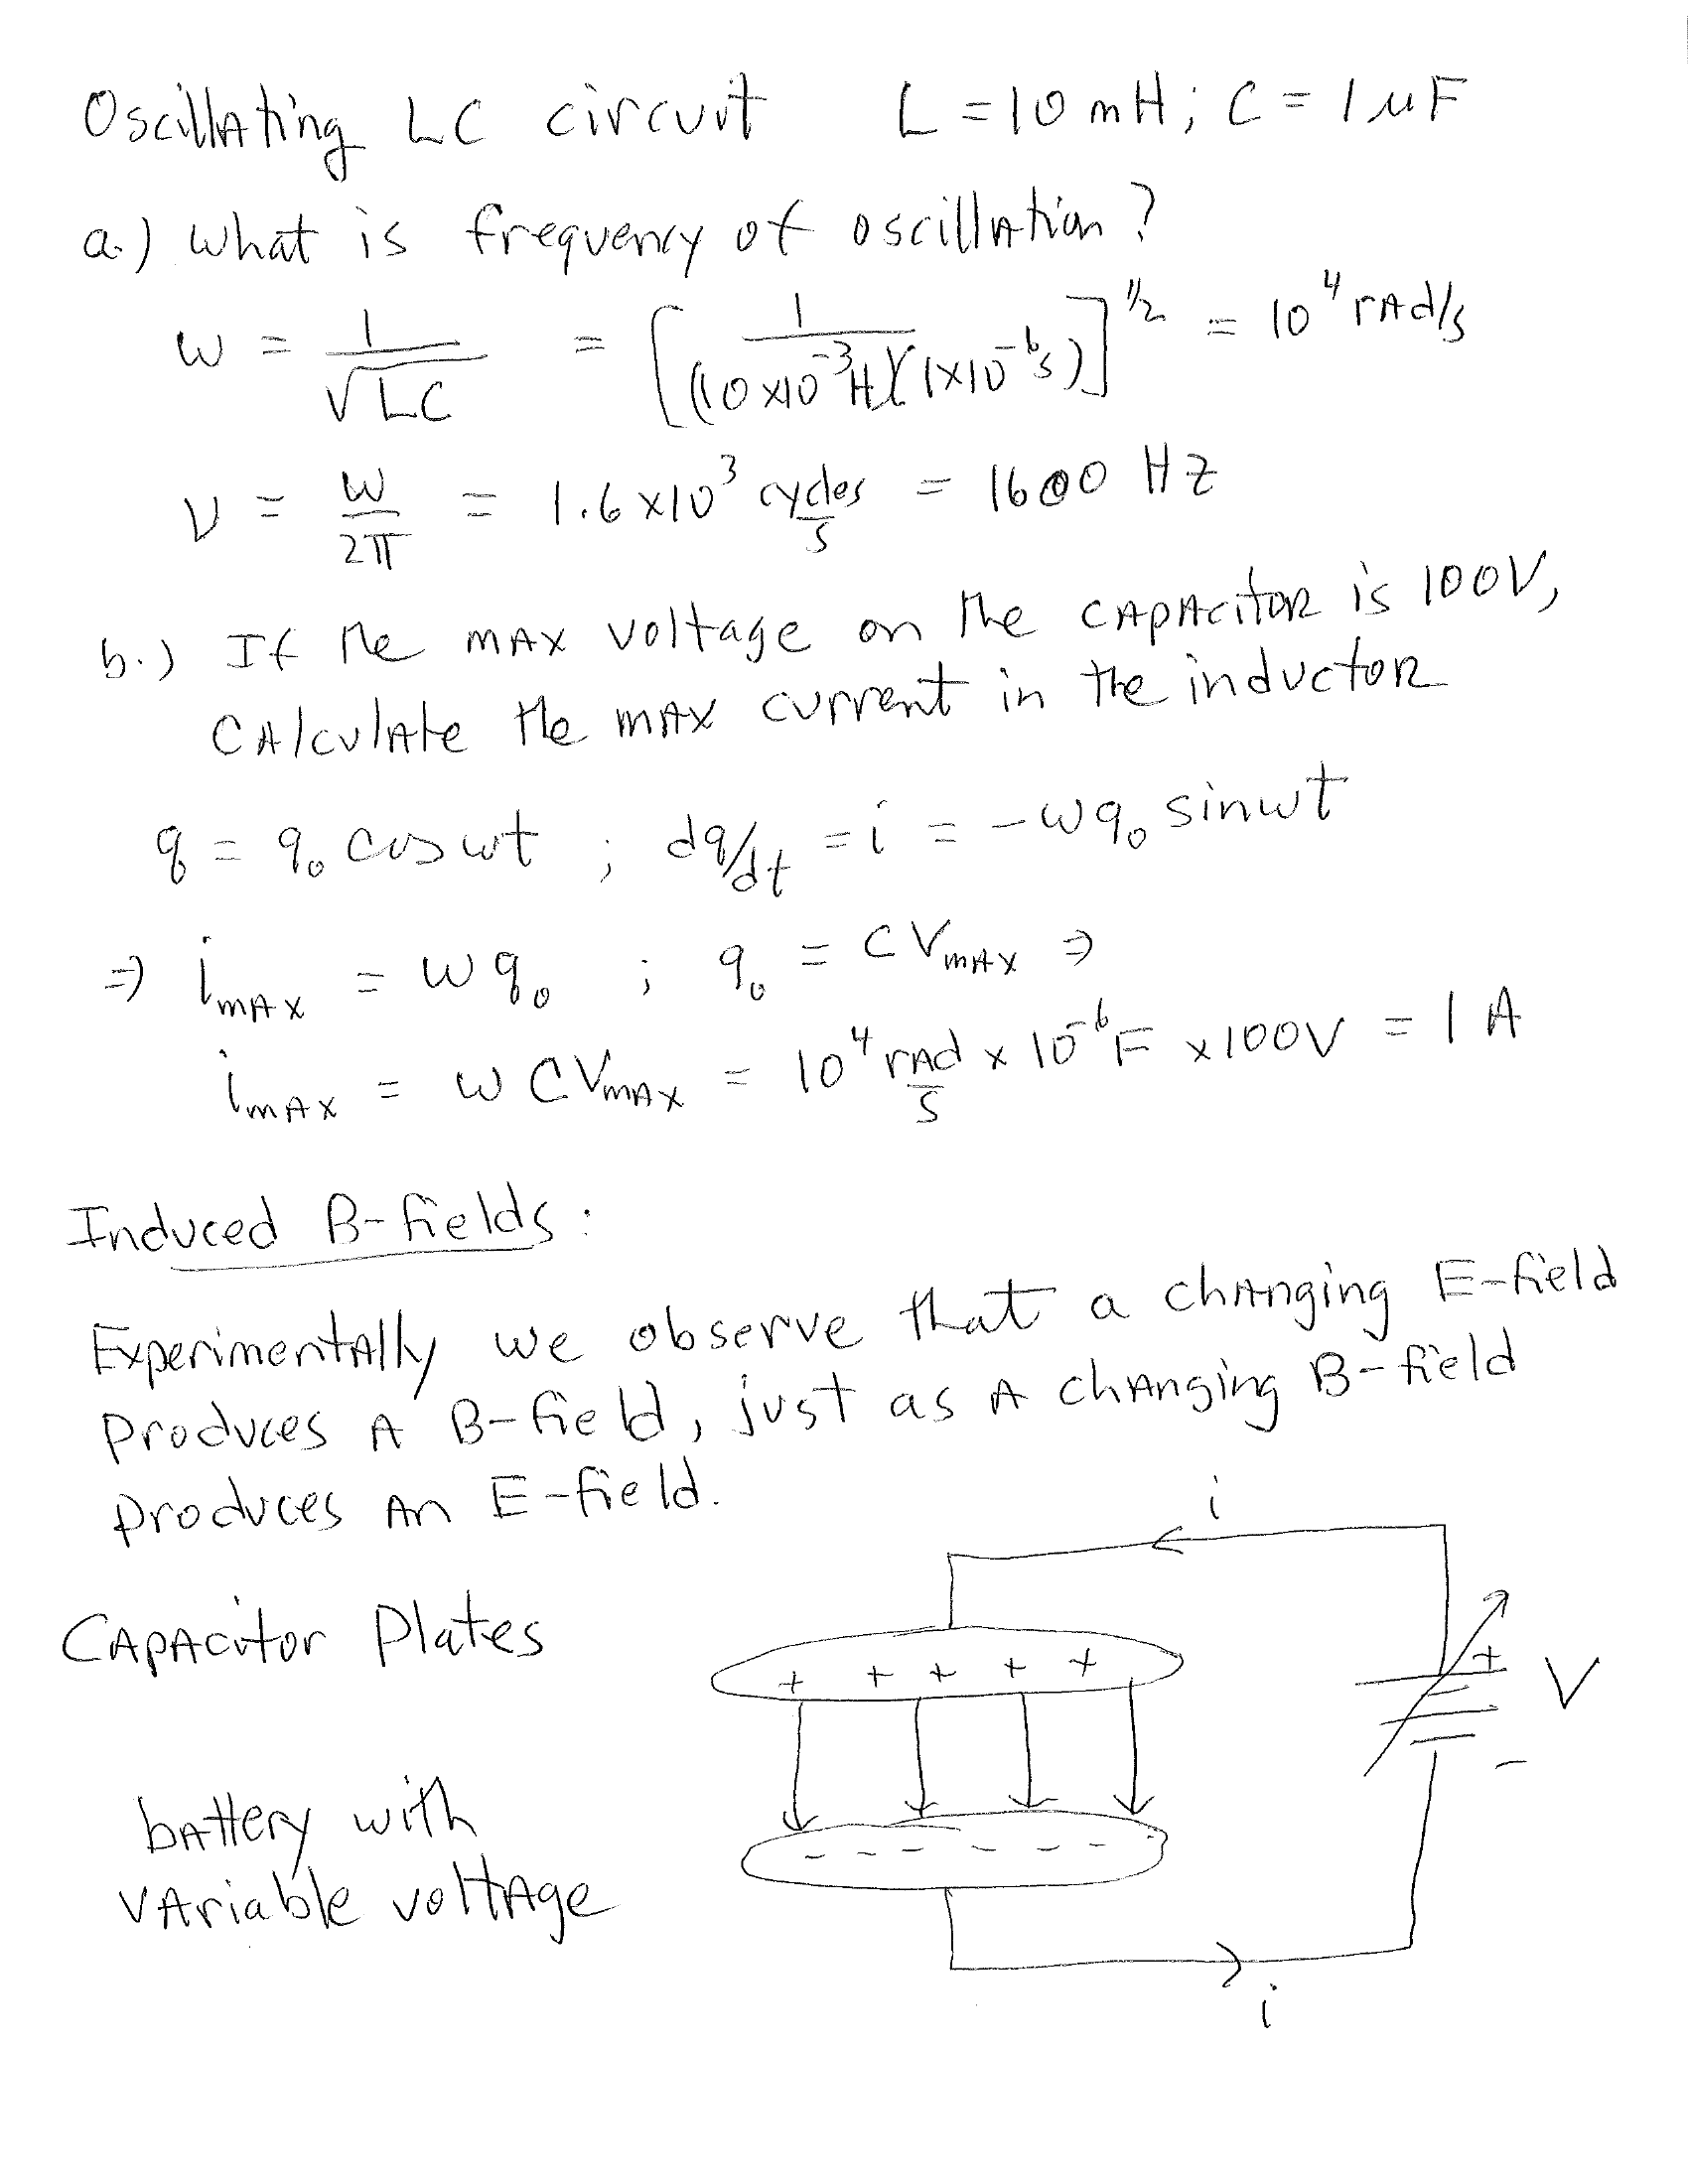
\includegraphics[width=0.9\textwidth,keepaspectratio]{figures/unit_10/page-4.png}
  \caption*{Unit 10, page 4}
\end{figure}
\clearpage
\begin{figure}[p]
  \centering
  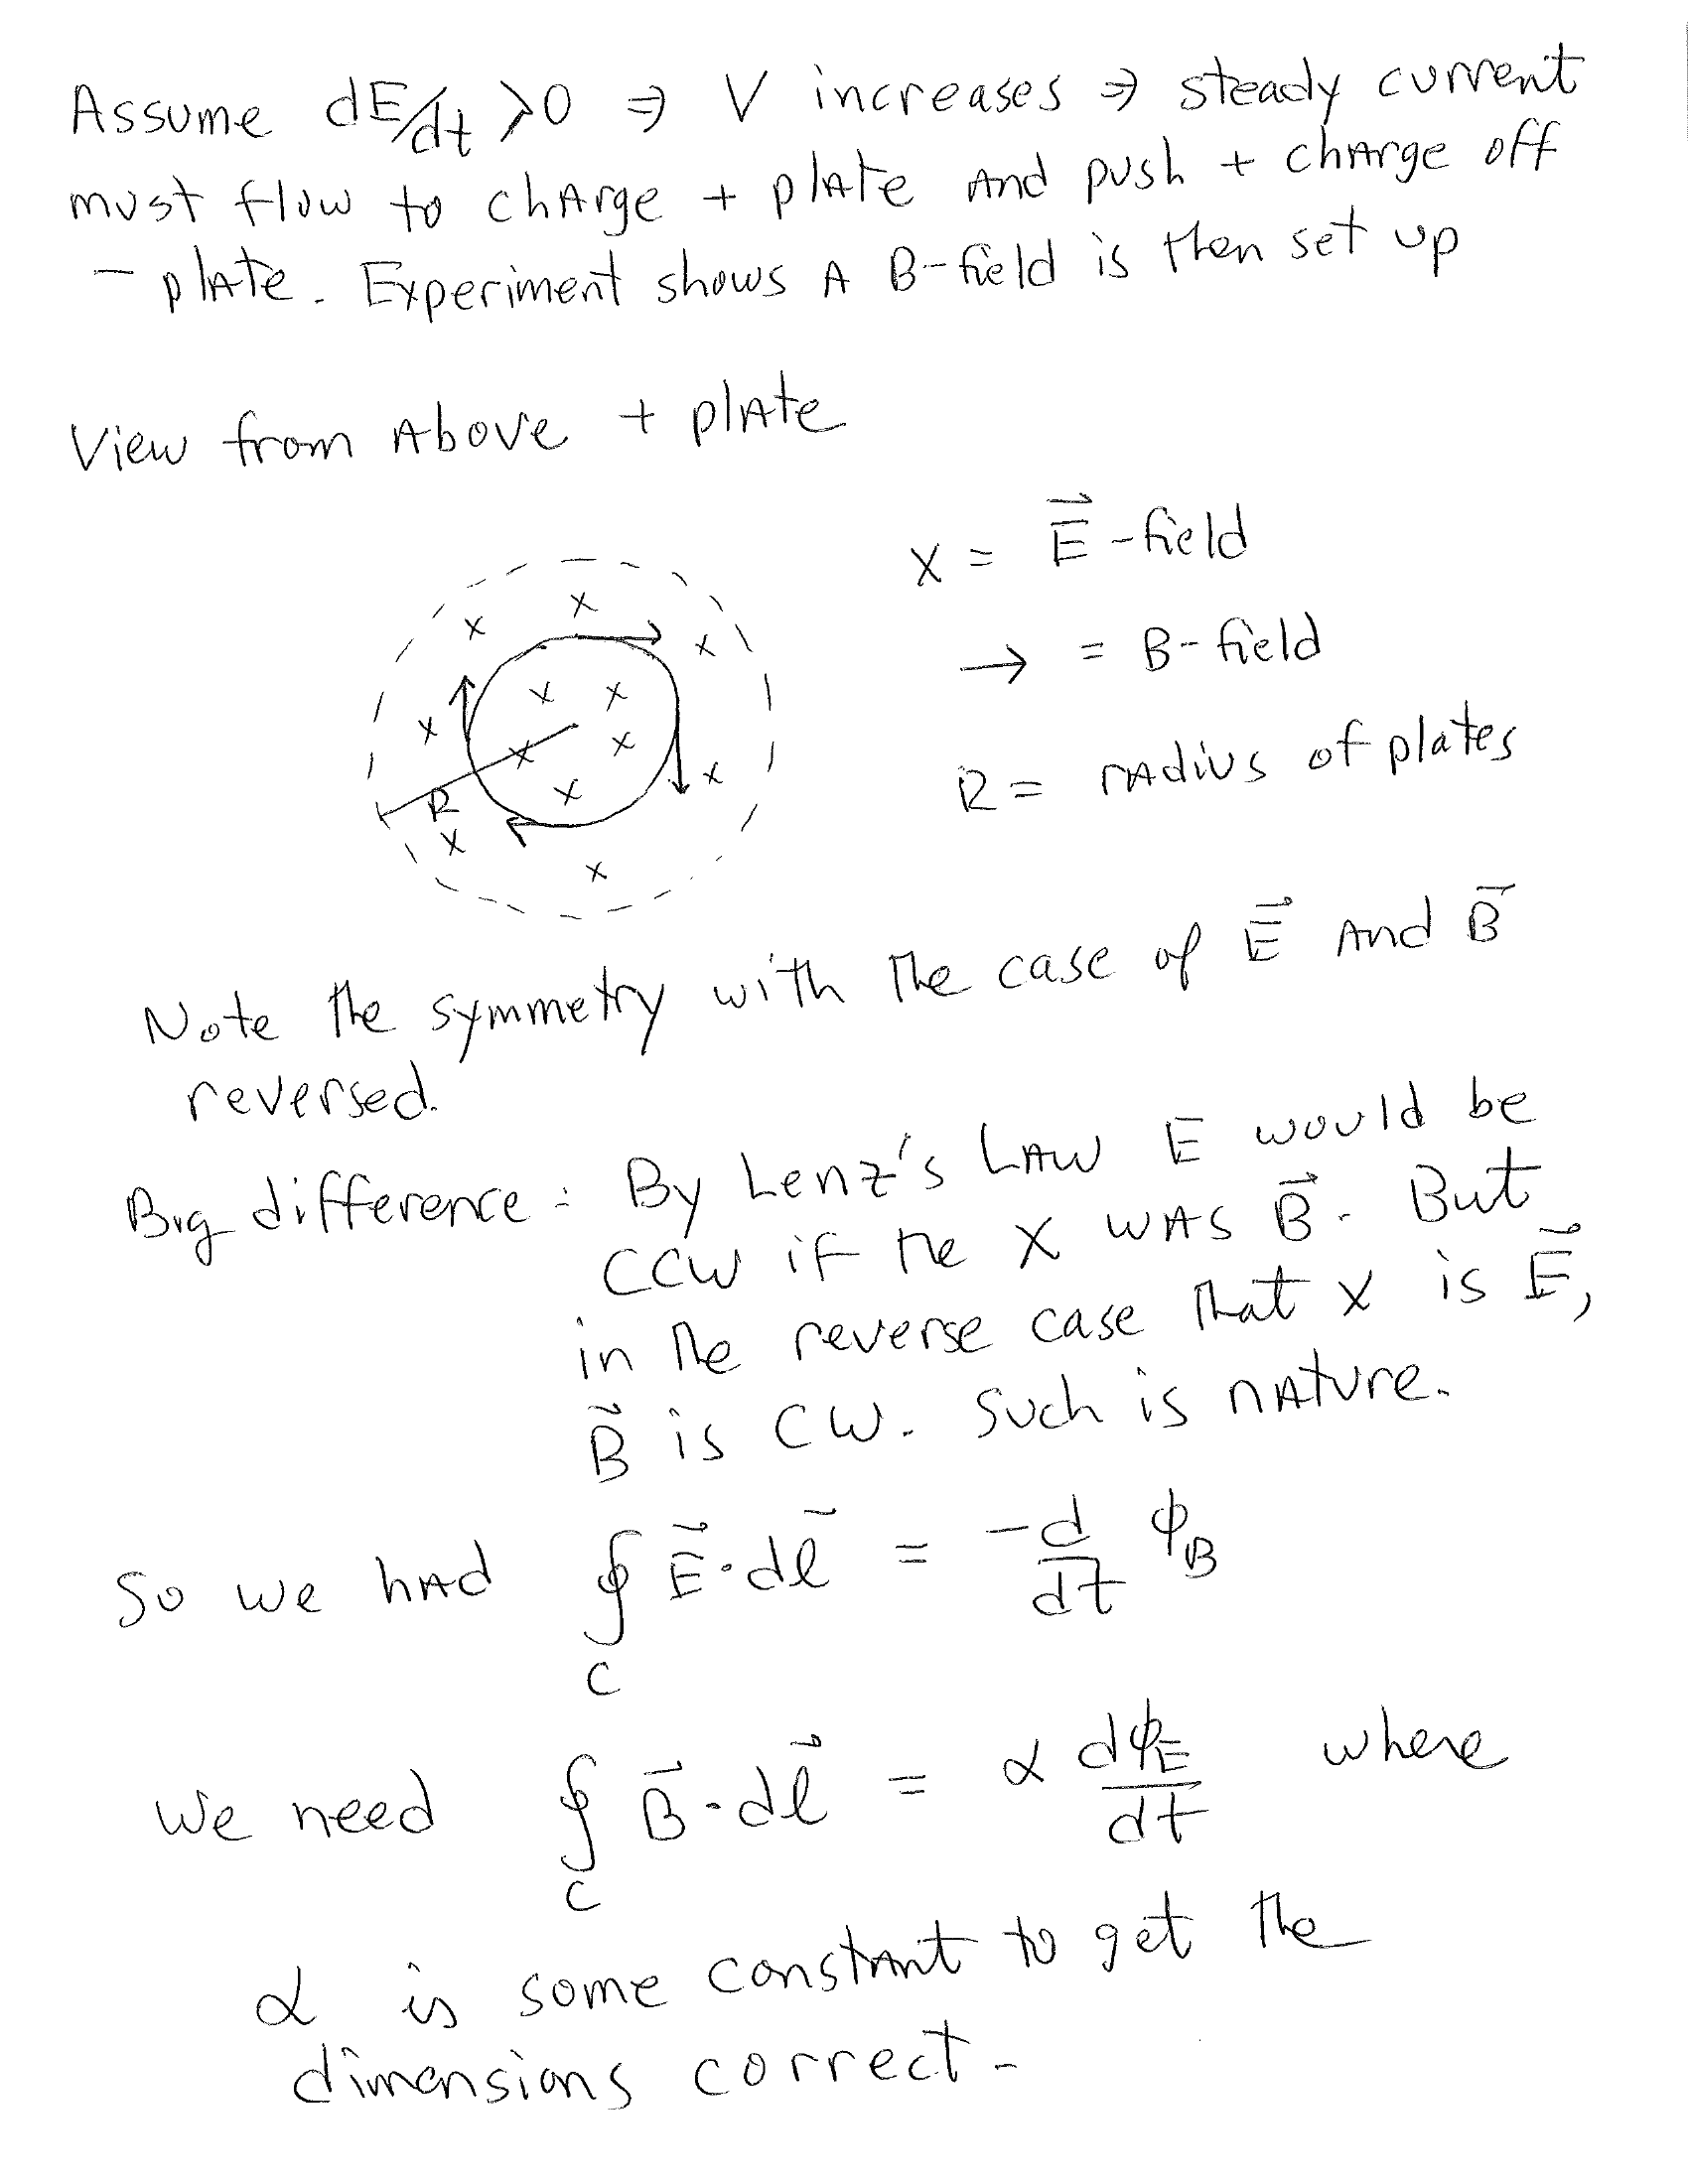
\includegraphics[width=0.9\textwidth,keepaspectratio]{figures/unit_10/page-5.png}
  \caption*{Unit 10, page 5}
\end{figure}
\clearpage
\begin{figure}[p]
  \centering
  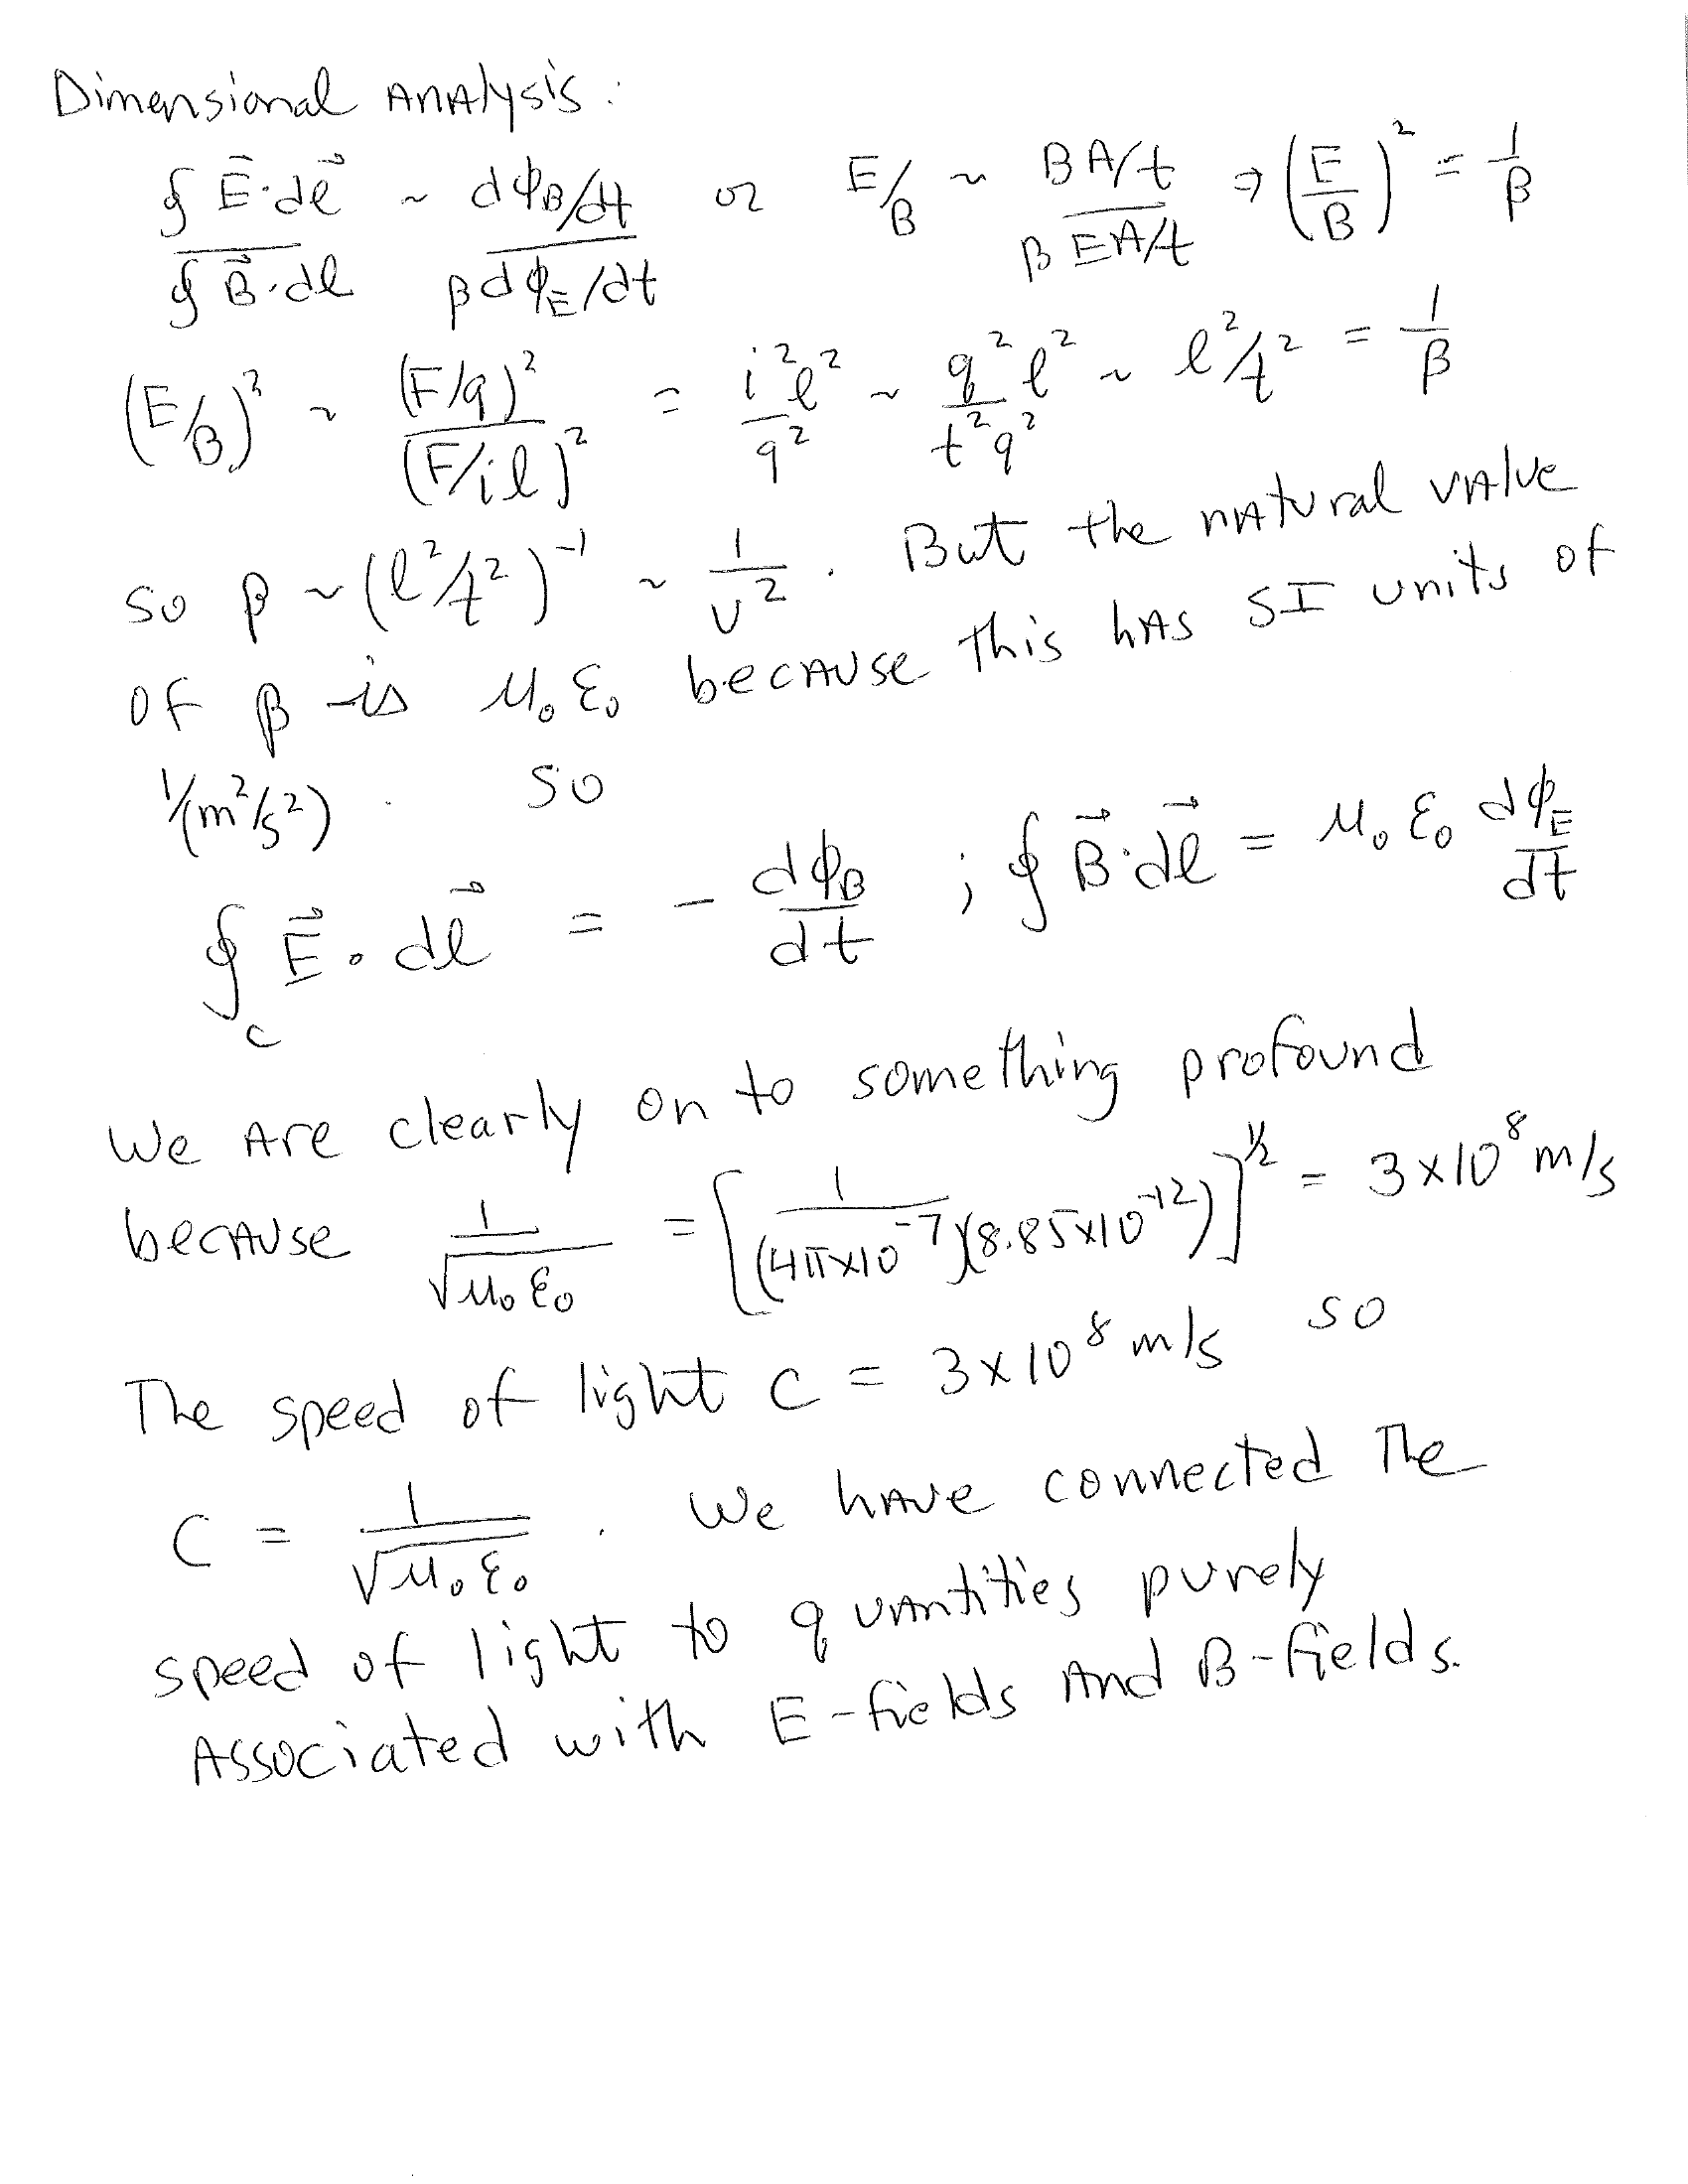
\includegraphics[width=0.9\textwidth,keepaspectratio]{figures/unit_10/page-6.png}
  \caption*{Unit 10, page 6}
\end{figure}
\clearpage
\begin{figure}[p]
  \centering
  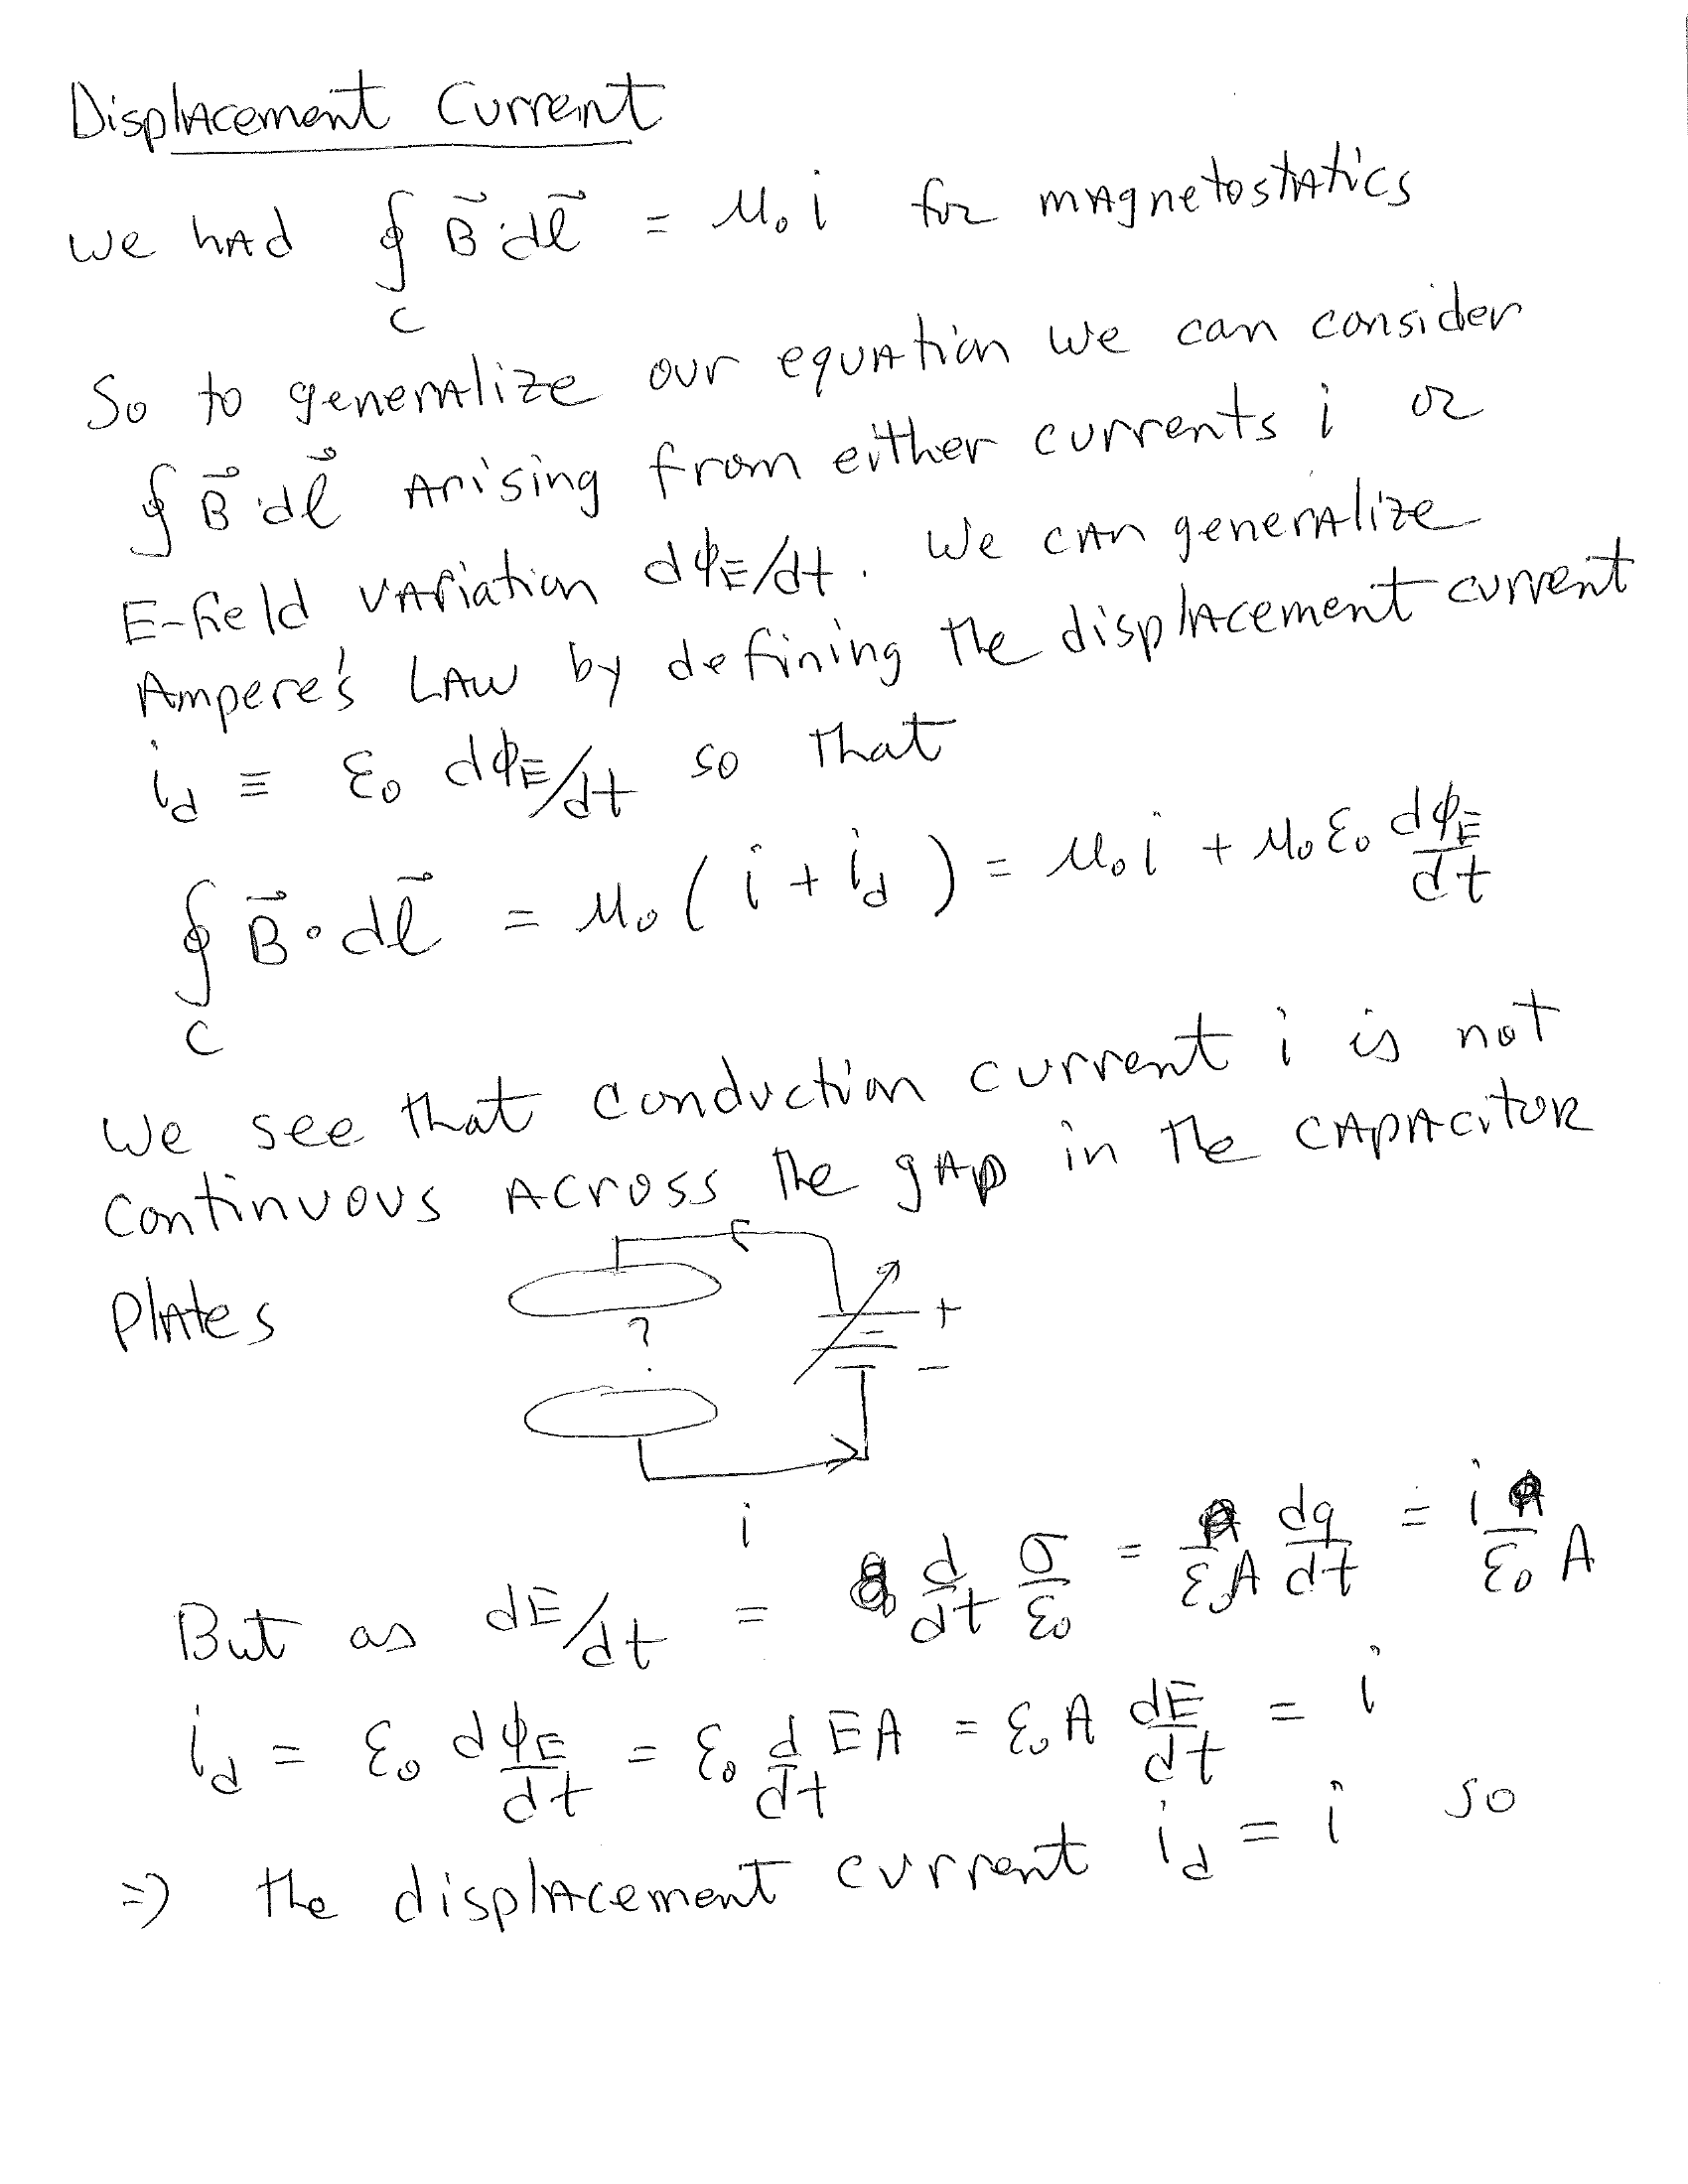
\includegraphics[width=0.9\textwidth,keepaspectratio]{figures/unit_10/page-7.png}
  \caption*{Unit 10, page 7}
\end{figure}
\clearpage
\begin{figure}[p]
  \centering
  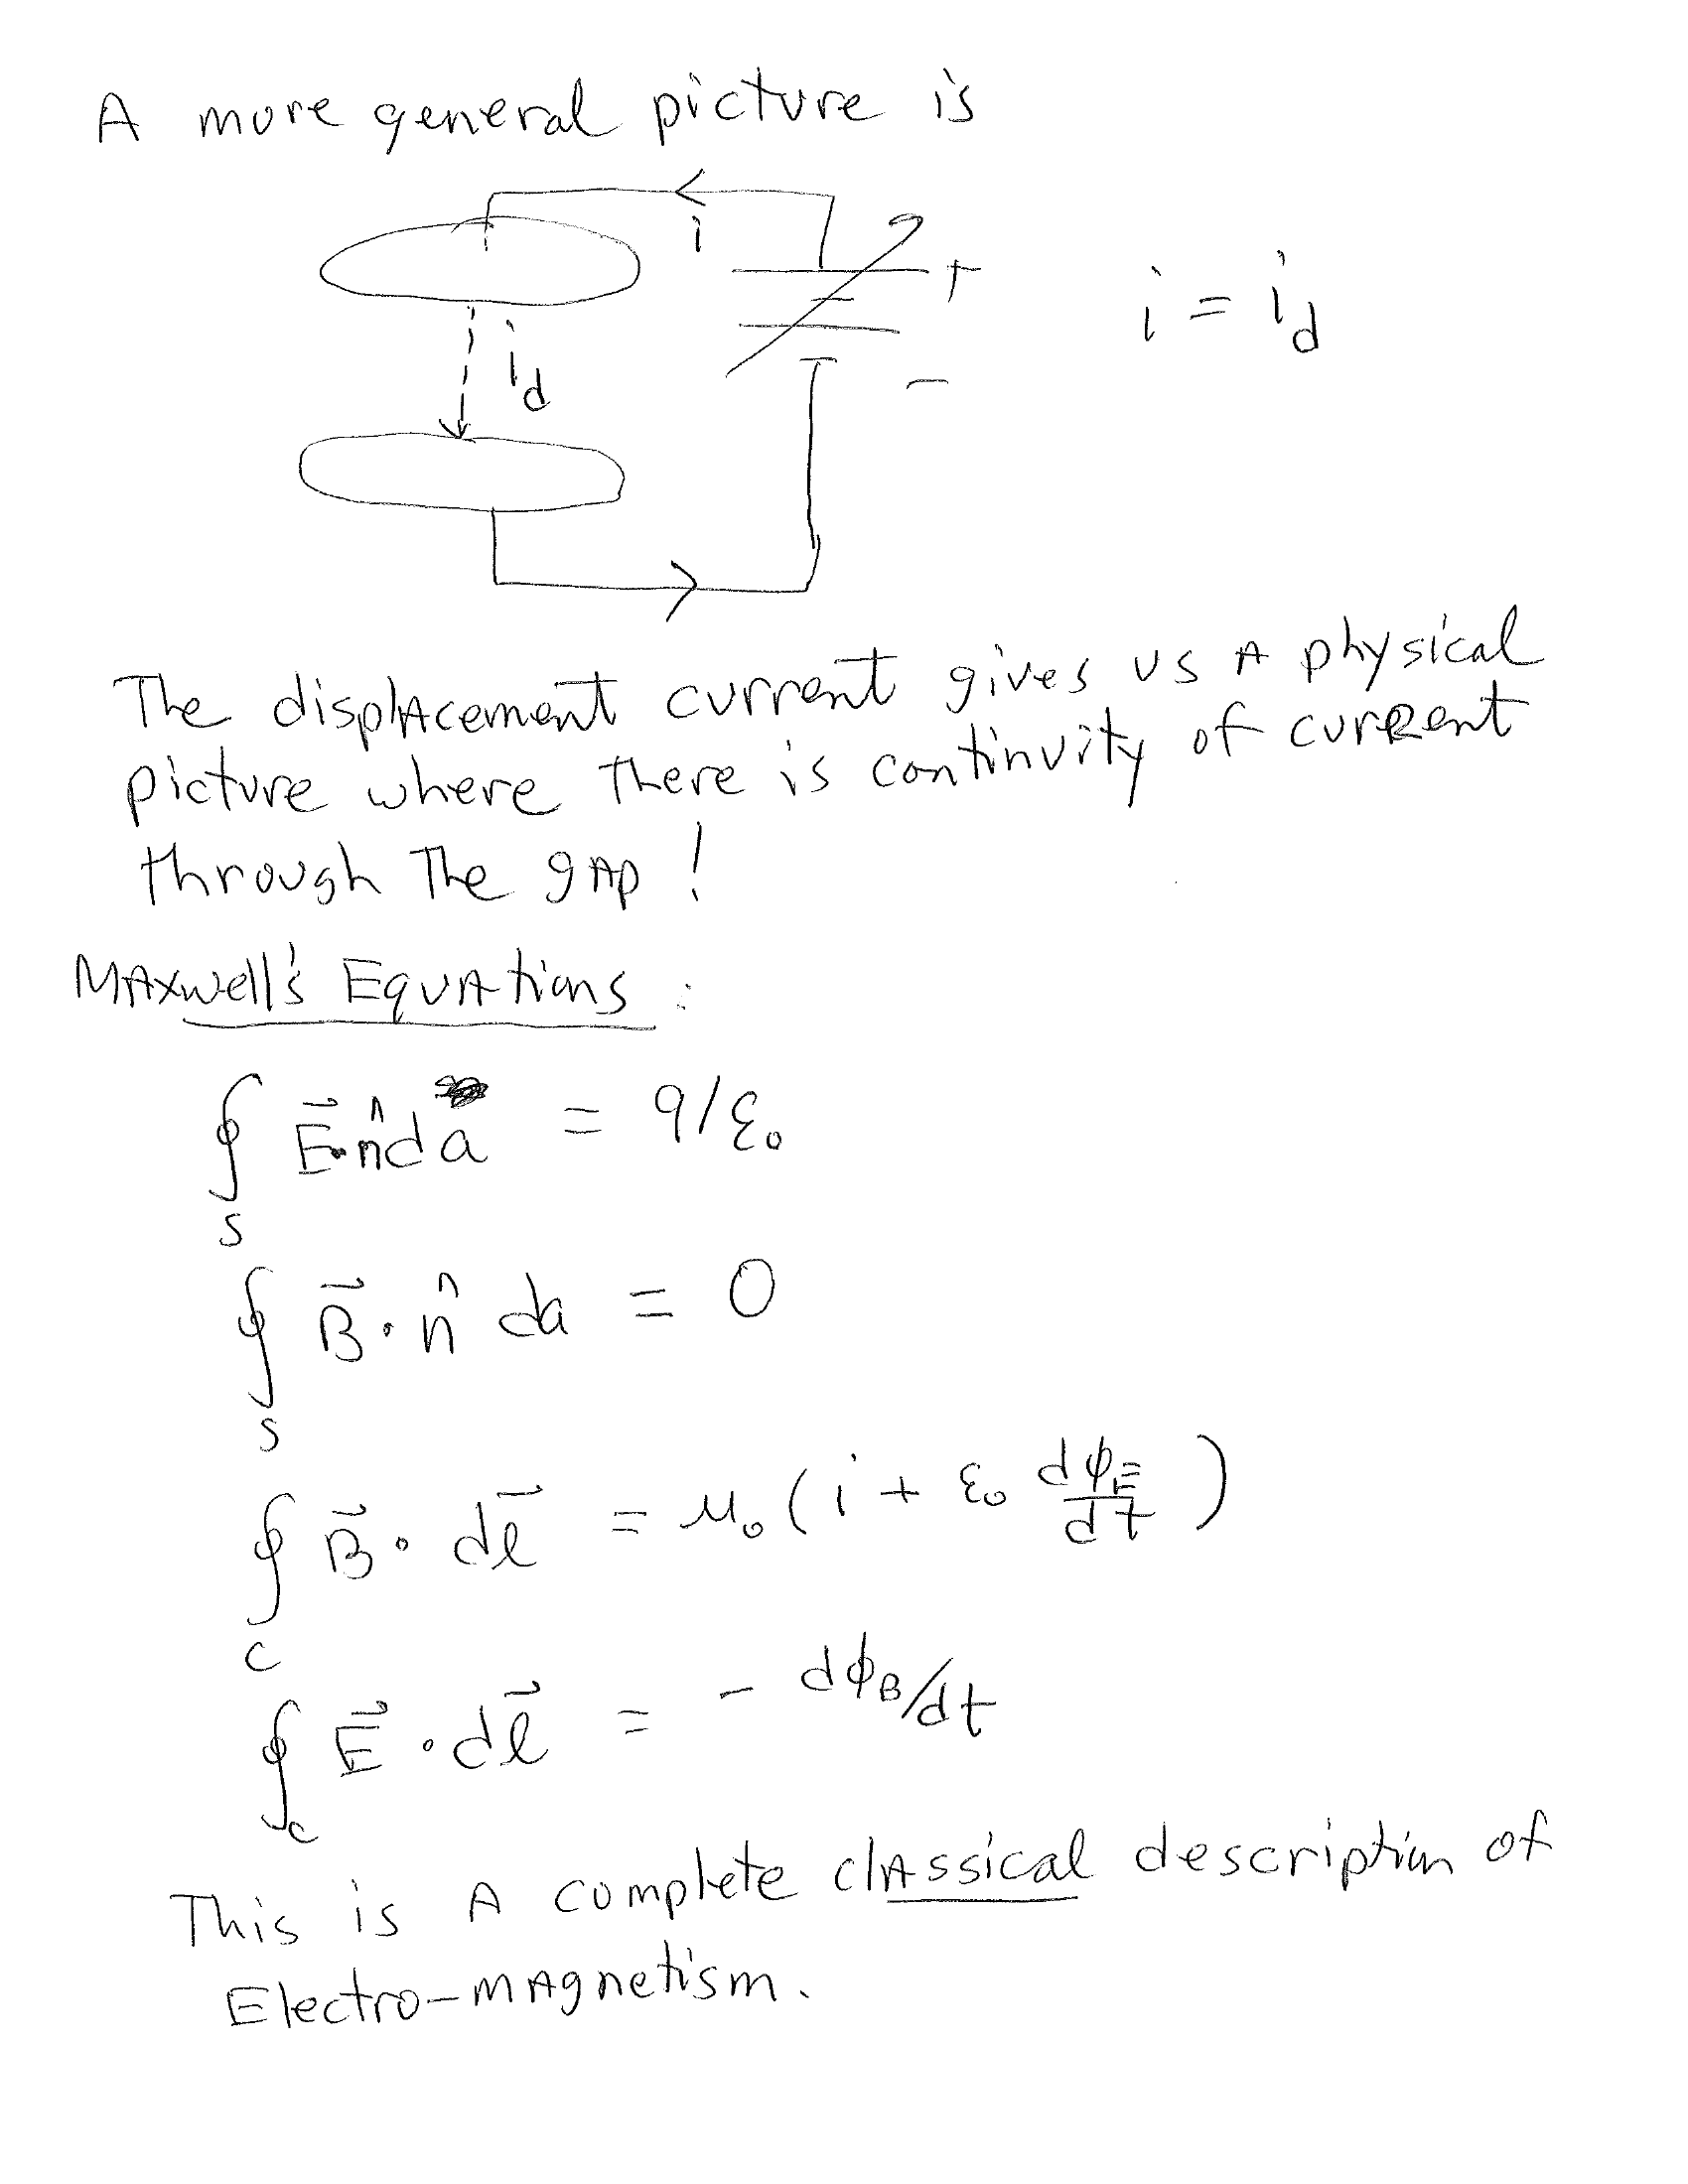
\includegraphics[width=0.9\textwidth,keepaspectratio]{figures/unit_10/page-8.png}
  \caption*{Unit 10, page 8}
\end{figure}
\clearpage
